\documentclass[12pt]{article}
\usepackage[utf8]{inputenc}
\usepackage{cite}
\usepackage[spanish]{babel}
\selectlanguage{spanish}
\usepackage{graphicx}
\graphicspath{ {files/} }
\usepackage{url}
\usepackage{natbib}
\usepackage[table,xcdraw]{xcolor}
\usepackage{float}
\usepackage{wrapfig}
\usepackage{paracol}
\usepackage{tensor}
\usepackage{amssymb}
\usepackage{amsmath}



\title{Reporte sobre la Evaluaci\'on 2}
\author{García Parra Pedro Antonio}
\date{Mayo 2019}

\begin{document}

\maketitle
Esta evaluaci\'on se basa en el concepto de la \textit{Evapotranspiraci\'on}. En la planeaci\'on de irrigaci\'on de cultivos o estudios de uso de agua en la Agricultura, se requiere conocer la cantidad de vapor de agua en la atm\'osfera que proviene por un lado de la evaporaci\'on de la humedad de suelo, as\'i como tambi\'en de la transpiraci\'on de las plantas. A este proceso se le conoce como \textit{Evapotranspiraci\'on}.\\
El m\'etodo que utiliz\'o la Organizaci\'on de las Naciones Unidas para la Alimentaci\'on y la Agricultura para modelar la \textit{Evapotranspiraci\'on} fue la ecuaci\'on de Penman-Monteith. La \textit{Evapotranspiraci\'on} de referencia $ET_0$, es uno de los par\'ametros mas importantes en los estudios hidrol\'ogicos, ambientales y agr\'icolas y juega un papel muy importante en los proyectos de manejo de irrigaci\'on y uso de agua en la agricultura. \\ 
El requerimiento de conocer un conjunto de valores de las variables climáticas ha sido una de las limitantes de la aplicación de la Ecuación de Penman-Monteith. Por ello se han desarrollado toda una serie de ecuaciones para el cálculo alternativo de la $ET_0$ bajo diversas condiciones climáticas.\\

Para realizar la evaluaci\'on utilizamos dos archivos de datos que conten\'ian datos metereol\'ogicos y de flujo, respectivamente. La evaluaci\'on se separ\'o en tres partes. En la \textbf{primera parte} se nos pide crear una tabla similar a la  \textit{Tabla 1} del articulo de \textit{Koffi Djaman}. Esta tabla deb\'ia contener los valores promedio mensuales de ciertas variables que posteriormente usaremos para encontrar el valor de $ET_0$.\\
Contru\'i la tabla \textit{(Cuadro \ref{tab:tabla1})} separando el dataframe que conten\'ia todos los datos del año en 12 dataframes que contenian cada uno los datos de un mes; sobre estos dataframes de mes realic\'e un loop que recorriera los datos y obtuviera los promedios de todas las variables necesarias.
Con esta tabla realic\'e tres gr\'aficas que muestran la variaci\'on mensaual de temperatura \textit{(figura \ref{fig:temp})}, humedad realativa \textit{(figura \ref{fig:hr})} y radiaci\'on solar \textit{(figura \ref{fig:rs})}\\
Para la \textbf{segunda parte} se nos pide que evaluemos tres ecuaciones:\\
\begin{itemize}
    \item 
        Jansen y Haise:
        $$ET_0 = (0.0252T + 0.078)Rs$$
        donde T es la temperatura promedio.
    \item
        Valiantzas 1:
        \begin{equation*}
        \begin{split}
        ET_0 = \ &0.0393Rs(Tmean + 9.5)^{0.5} - 0.19Rs^{0.6}\phi^{0.15} + \\
                 &0.0061(Tmean + 20)(1.12 \ Tmean - Tmin - 2)^{0.7}
        \end{split}
        \end{equation*}

    \item
        Valiantzas 4:
        \begin{equation*}
        \begin{split}
            ET_0 = \ &0.051(1-\alpha)Rs(Tmean + 9.5)^{0.5} - 2.4(Rs/R_a)^2 + \\
                     &0.048(Tmean + 20)(1 - RH/100)(0.5 + 0.536u_2) + 0.00012z
        \end{split}
        \end{equation*}
    \end{itemize}

La ecuaci\'on \textit{Valiantzas 4} requiere otras 4 ecuaciones extras:

        \begin{equation*}
        \begin{split}
            R_a &= \frac{24(60)}{\pi}G_{se}d_r[\omega_s\sin{\phi}\sin{\delta} + \cos{\phi}\cos{\delta}\sin{\omega_s}]\\
            \omega_s &= \arccos[-\tan\phi\tan\delta]\\
            \delta &= 0.409\sin{(\frac{2\pi}{365}J - 1.39)}\\
            d_r &= 1 + 0.033\cos{(\frac{2\pi}{365}J)}
        \end{split}
        \end{equation*}
        
Para realizar la tarea primero cree funciones para calcular cada uno de los datos anteriores:
\begin{verbatim}
    def d(J):
        return 1+0.033*np.cos(2/365*np.pi*J)
    
    def delta(J):
        return 0.409*np.sin(2*np.pi/365*J - 1.39)
    
    def w(s):
        lat = 0.504725
        return np.arccos(-1*np.tan(lat)*np.tan(delta(s)))
        
    def Ra(j):
        lat = 0.504725
        return 24*60/np.pi*(0.082)*d(j)*(w(j)*np.sin(lat) * 
        np.sin(delta(j)) + np.cos(lat)*np.sin(w(j)))
    
    def JH(t,rs):
        return (0.0252*t + 0.078) * rs
    
    def val1(rs,tmean,phi,tmin):
        return ( 0.0393*rs*((tmean + 9.5)**(0.5)) - 
                 0.19*rs**(0.6) * phi**(0.15) + 0.0061 * 
                 (tmean + 20) * (1.12*tmean - tmin - 2)**(0.7) )
    def val4(a,rs,tmean,dia,rh,u2,z):
        return (0.051*(1-a)*rs*(tmean + 9.5)**(0.5) - 
                2.4*(rs/Ra(dia))**2 + 0.048*(tmean + 20)*(1 - 
                rh/100)*(0.5 + 0.536*u2) + 0.00012*z)
\end{verbatim}
Primero obtuve el promedio de los datos por d\'ia y los guarde en un dataframe que llam\'e df2Dia para sobre este dataframe utilizar las funciones y obtener los valores de $ET_0$. Esto me consigu\'o el valor diario de $ET_0$, ahora saqu\'e el promedio mensual y lo guarde en otro dataframe (\textit{Cuadro \ref{tab:tabla2}}).\\

Para la \textbf{parte tres} se utiliz\'o el segundo archivo de datos y el objetivo era replicar la grafica que se aprecia en la \textit{figura \ref{fig:ejemplo}} donde se promedien los datos de un mes por horas. Primero, tras leer el archivo de datos y obtener un dataframe, obtuve la fecha completa ya que los datos estan tomados de manera que el d\'ia es un n\'umero entre el 1 y 365; y la agregu\'e al dataframe:
\begin{verbatim}
    DATA=(np.asarray(df1['Year']-1970, dtype='datetime64[Y]')) + 
         (np.asarray(df1["DoY"], dtype='timedelta64[D]')-1)
    df1["FECHA"] = DATA
\end{verbatim}
Al tener la fecha en formato estandar, pude cortar el dataframe de manera que tuviera s\'olo un mes (utilic\'e el mes de abril) y posteriormente utilic\'e la funcion \texttt{groupby()} junto con \texttt{.transform("mean")} de pandas para obtener el promedio por hora de los datos de todo el mes.\\
El resultado puede verse en la \textit{figura \ref{fig:flujo}}.
\begin{table}[]
\centering
\resizebox{\textwidth}{!}{%
\begin{tabular}{l|ccccccccccc}
 & Elevación (m) & Latitud (rad) & Longitud (rad) & RHmax & RHmean & RHmin & Rs & Tmax & Tmean & Tmin & VelViento \\ \hline
\rowcolor[HTML]{EFEFEF} 
Enero & 101 & 0.504725 & 1.942737 & 91.60 & 38.450544 & 5.98 & 34.802554 & 33.35 & 16.971598 & 0.54 & 1.944333 \\
Febrero & 101 & 0.504725 & 1.942737 & 99.53 & 48.168006 & 6.76 & 56.250350 & 31.47 & 17.230275 & 0.07 & 1.964189 \\
\rowcolor[HTML]{EFEFEF} 
Marzo & 101 & 0.504725 & 1.942737 & 89.73 & 36.968353 & 6.76 & 92.894913 & 35.22 & 19.282359 & 3.06 & 1.926196 \\
Abril & 101 & 0.504725 & 1.942737 & 93.40 & 40.785667 & 5.23 & 134.012965 & 36.30 & 21.880618 & 5.43 & 2.101812 \\
\rowcolor[HTML]{EFEFEF} 
Mayo & 101 & 0.504725 & 1.942737 & 94.60 & 44.233468 & 8.19 & 162.405343 & 38.18 & 23.650034 & 7.13 & 2.113918 \\
Junio & 101 & 0.504725 & 1.942737 & 98.37 & 50.810507 & 5.34 & 163.926069 & 41.47 & 28.416187 & 13.12 & 2.154986 \\
\rowcolor[HTML]{EFEFEF} 
Julio & 101 & 0.504725 & 1.942737 & 97.00 & 57.639805 & 13.10 & 157.534402 & 44.94 & 31.065726 & 18.71 & 2.022204 \\
Agosto & 101 & 0.504725 & 1.942737 & 98.60 & 68.868454 & 30.16 & 151.273589 & 40.24 & 30.120894 & 22.71 & 1.910853 \\
\rowcolor[HTML]{EFEFEF} 
Septiembre & 101 & 0.504725 & 1.942737 & 98.03 & 66.619750 & 21.32 & 136.749910 & 41.39 & 29.661271 & 19.43 & 1.790326 \\
Octubre & 101 & 0.504725 & 1.942737 & 98.47 & 68.696082 & 17.32 & 95.513468 & 35.82 & 23.254207 & 10.23 & 1.664435 \\
\rowcolor[HTML]{EFEFEF} 
Noviembre & 101 & 0.504725 & 1.942737 & 99.43 & 58.085458 & 8.75 & 60.384285 & 32.39 & 16.966396 & 2.47 & 1.498097 \\
Diciembre & 101 & 0.504725 & 1.942737 & 97.33 & 58.333938 & 8.04 & 44.962366 & 31.86 & 14.332823 & -1.34 & 1.628730
\end{tabular}%
}
\caption{Tabla de promedios mensuales de temperatura, humedad relativa, radiaci\'on solar y velocidad del viento.}
\label{tab:tabla1}
\end{table}
\begin{table}[]
\centering
\resizebox{\textwidth}{!}{%
\begin{tabular}{l|ccc}
 & Jensen and Haise  & Valiantzas 1 & Valiantzas 4 \\ \hline
\rowcolor[HTML]{EFEFEF} 
Enero & 16.649192 & 6.844436 & 8.381659 \\
Febrero & 27.831158 & 10.302332 & 11.581779 \\
\rowcolor[HTML]{EFEFEF} 
Marzo & 52.703909 & 18.273990 & 16.720430 \\
Abril & 84.551798 & 27.715380 & 23.899589 \\
\rowcolor[HTML]{EFEFEF} 
Mayo & 109.611487 & 34.607619 & 30.298015 \\
Junio & 130.542559 & 37.566474 & 37.198765 \\
\rowcolor[HTML]{EFEFEF} 
Julio & 136.149008 & 37.291964 & 29.017621 \\
Agosto & 127.498420 & 35.266665 & 29.237869 \\
\rowcolor[HTML]{EFEFEF} 
Septiembre & 113.434775 & 31.688309 & 24.737334 \\
Octubre & 64.226712 & 20.047382 & 16.862898 \\
\rowcolor[HTML]{EFEFEF} 
Noviembre & 30.923798 & 11.296789 & 12.397176 \\
Diciembre & 20.156472 & 7.927049 & 7.298170
\end{tabular}%
}
\caption{Tabla de los valores de $ET_0$ obtenidos con diferentes ecuaciones}
\label{tab:tabla2}
\end{table}

\begin{figure}
    \centering
    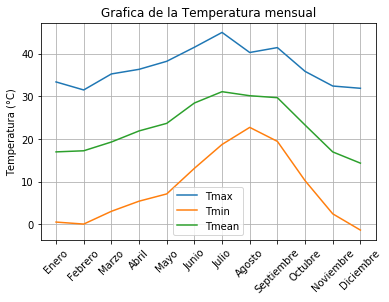
\includegraphics[scale = .8]{grafTemp.png}
    \caption{Grafica que muestra la variaci\'on promedio de la temperatura del año 2018}
    \label{fig:temp}
\end{figure}

\begin{figure}
    \centering
    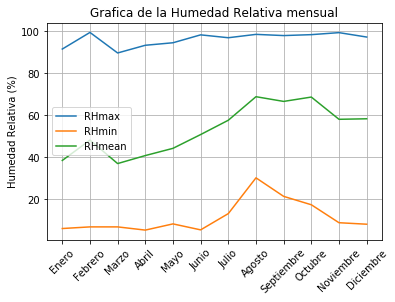
\includegraphics[scale = .8]{grafHR.png}
    \caption{Grafica que muestra la variaci\'on promedio de la humedad relativa del año 2018}
    \label{fig:hr}
\end{figure}

\begin{figure}
    \centering
    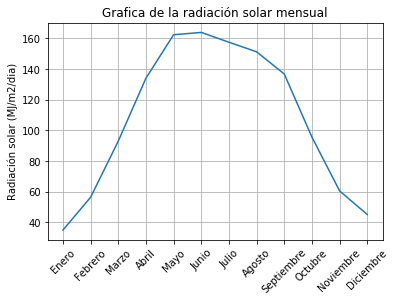
\includegraphics[scale = .8]{grafRS.png}
    \caption{Grafica que muestra la variaci\'on promedio de la radiaci\'on solar del año 2018}
    \label{fig:rs}
\end{figure}
\begin{figure}
    \centering
    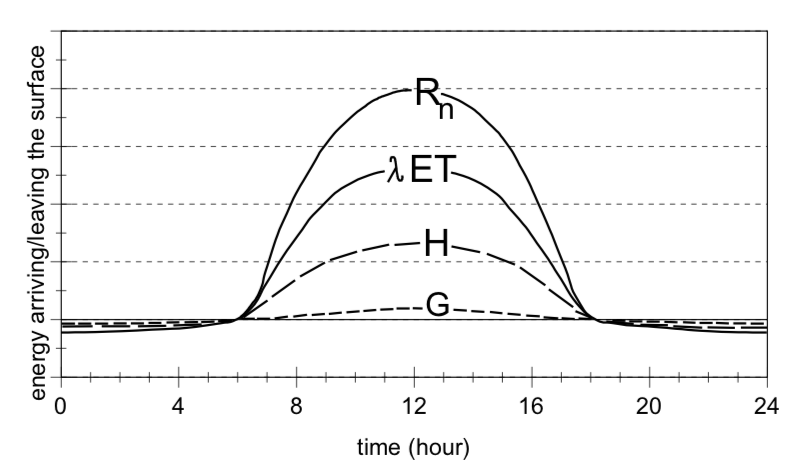
\includegraphics[scale = .5]{ejemplo.png}
    \caption{Grafica de ejemplo para la parte tres}
    \label{fig:ejemplo}
\end{figure}
\begin{figure}
    \centering
    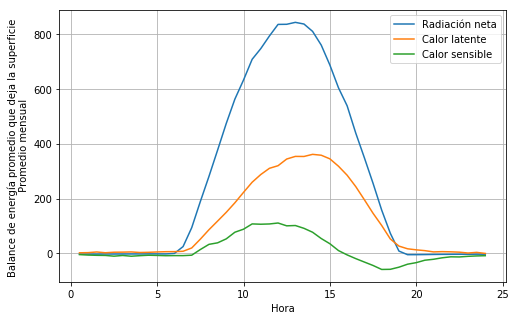
\includegraphics[scale = .8]{grafFlujo.png}
    \caption{Grafica del flujo de calor de todo el mes de Abril 2018 promediada por horas.}
    \label{fig:flujo}
\end{figure}
\end{document}
